\section{Phase 1: Analysis of MRI images dataset}

\subsubsection*{NIFTI protocol}

The NIFTI protocol stores the MRI scan images in 3D format with spatial information that allows the doctors to analyze images knowing the orientation along with some other metadata. Data is stored as vectors with voxel information, so the voxel is stored with its magnitude and its direction.

This project is using the nibabel \cite{nibabel} library to load and process MRI images from NIFTI files. The library loads NIFTI files and retrieves an in-memory object with the image data containing slices in a 3-dimensional array. Accessing slices is then as easy as using the three indexes in the array, where you can easily get a slice by using the slice number from your chosen axis.

\subsubsection*{Loading images}
Extract 2D images: Load 3D images and extract 2D slices from the original dataset, which will be depicted with code.

After loading NIFTI images with the nibabel library \dots

\begin{figure}[ht]
    \centering
    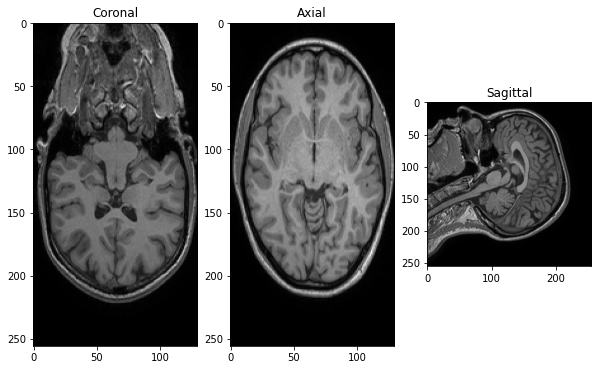
\includegraphics[width = 10cm, height = 6cm]{images/3-axis.png}
    \caption[Coronal, Axial and Sagittal images]{Coronal, Axial and Sagittal images}
    \label{fig:3-axis}
\end{figure}

Images are loaded in the following shape:

\begin{itemize}
    \item 256 slices of Coronal or trasversal plane 
    \item 256 slices of Axial or horizontal plane
    \item 130 slices of Sagittal
\end{itemize}

\subsubsection*{Deciding what slices to use}

Looking at the three different slices in Figure \ref{fig:3-axis}, it is obvious that images have not been processed to show only the brain but the whole skull. The aim of the project is to create artificial brain images, not head ones. A model that would learn head images would require much more time and resources than for learning just the brain (which is not an easy task at all either).

While observing the BraTS \cite{brats} challenge dataset and project description, the skull stripping concept arise. Skull stripping consists on removing anything that does not pertain to brain or, in other words, extract the brain from the skull. 

\begin{figure}[ht]
    \centering
    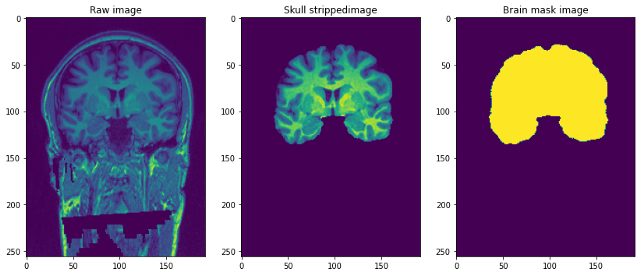
\includegraphics[width = 10cm, height = 6cm]{images/skull-stripped.png}
    \caption[Skull stripped image example]{Skull stripped image example; Source: Analytics Vidhya \cite{skullstripping} }
    \label{fig:skullstripped}
\end{figure}

This project cannot afford such implementation within the project scope. So, when deciding what slices to use, it became the only decision factor. It happened to be that the rest of considerations where just debatable and clearly much less important.

In conclusion, the noise that bones, eyes and the rest of the items visible in coronal and sagittal axis look very high compared to the axial slices in where, properly selected, slices will only show a surrounding skull bone.

Once that the axial slices were chosen, a sample of brain scans were visually analyzed to find a range of slices that could be used.

Figure \ref*{fig:slice160} shows a red line which bottom-up delimits  the range that goes from above the eyes to the top which is the range that excludes as much non-brain pixels as possible

\begin{figure}[ht]
    \centering
    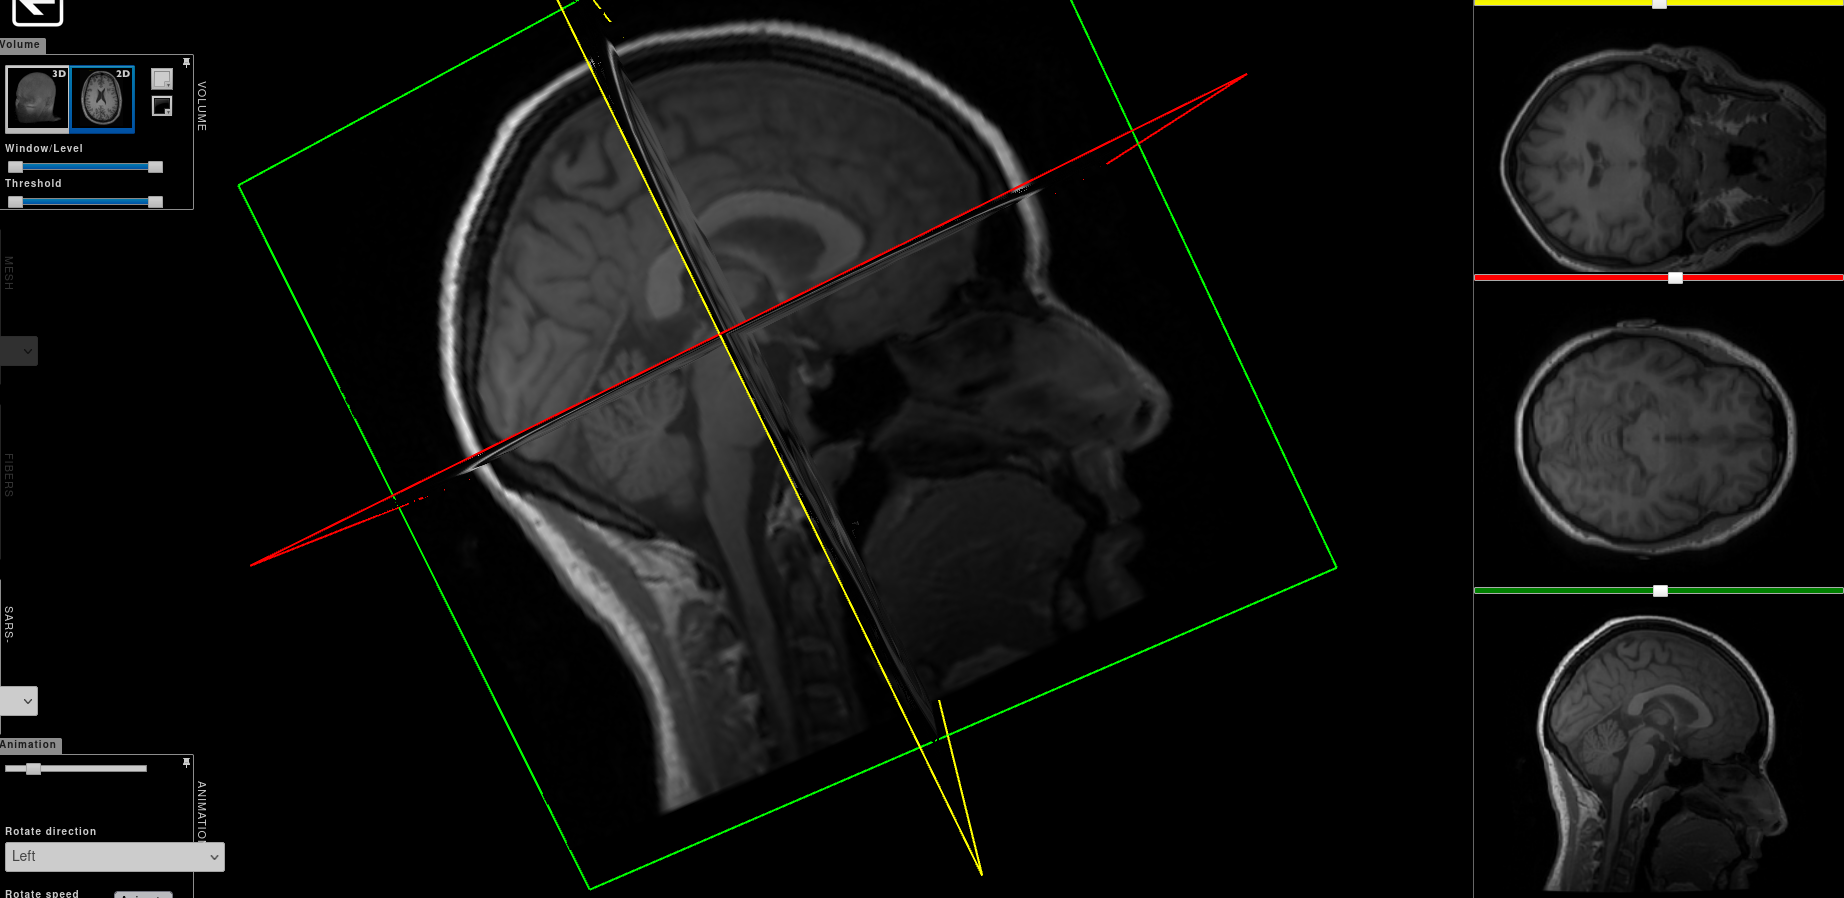
\includegraphics[width = 10cm, height = 6cm]{images/nifti-slice160.png}
    \caption[Slice 160 as bottom delimiter]{In red, slice 160 as bottom delimiter}
    \label{fig:slice160}
\end{figure}

Also, the slices closer to the top were also discarded to avoid higher heterogeneity on brain images (size and content). See Figure \ref*{fig:slice190}.

\begin{figure}[ht]
    \centering
    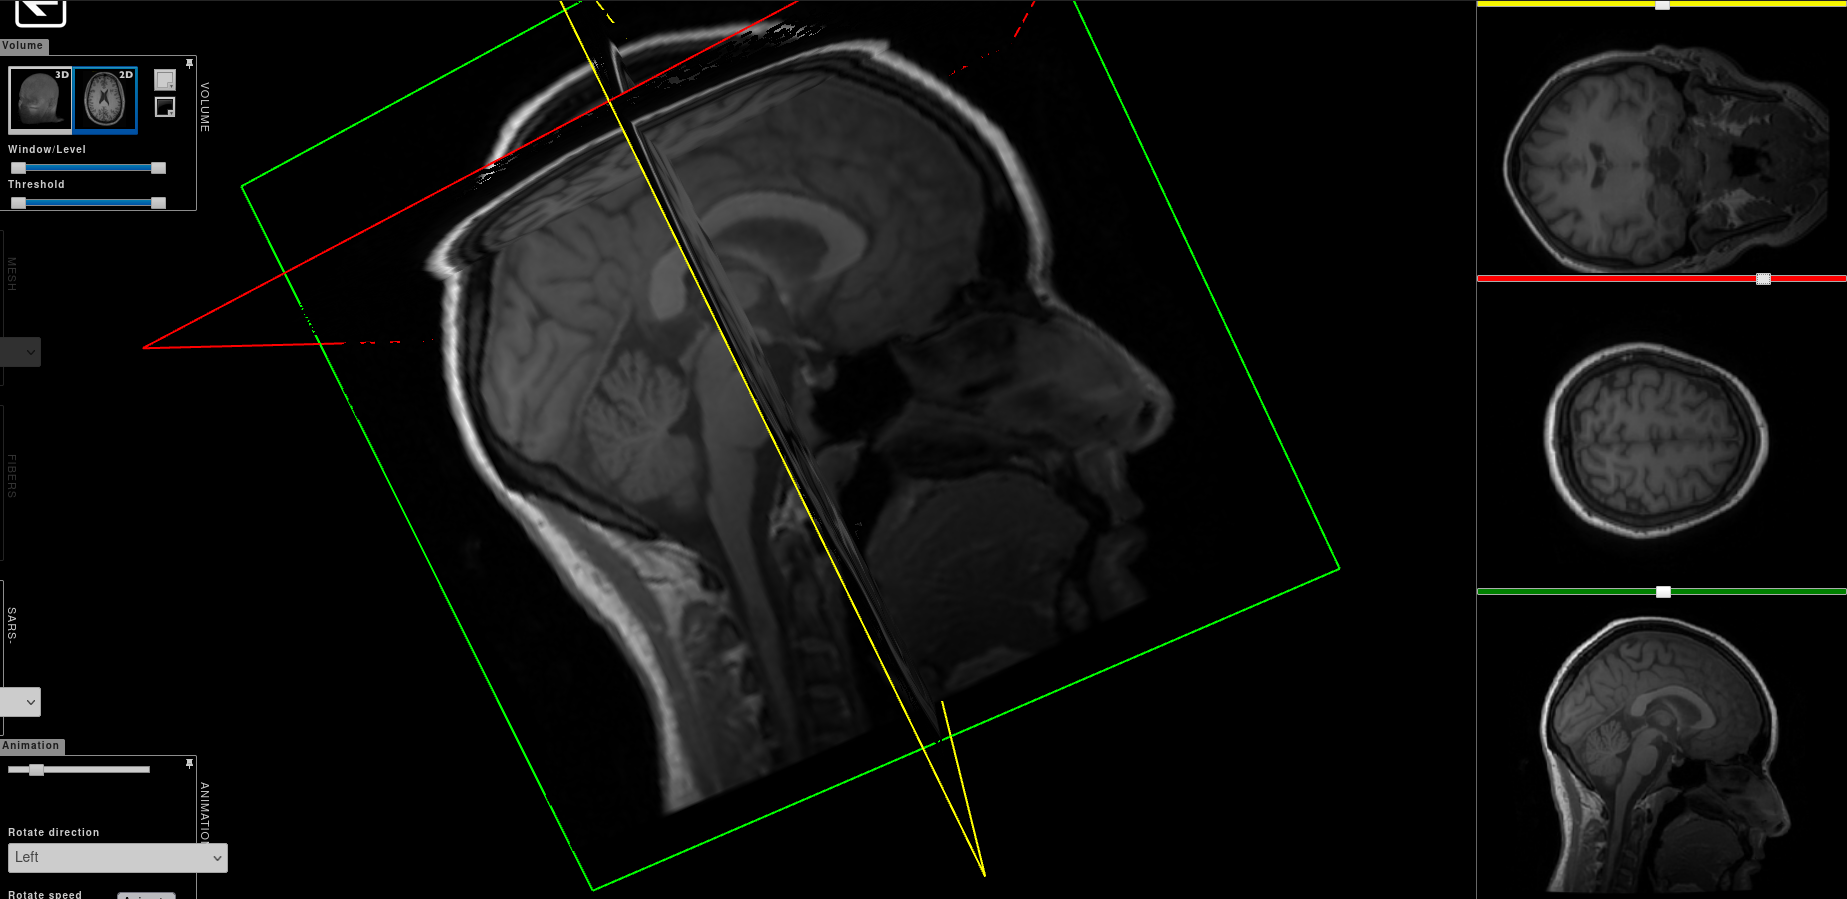
\includegraphics[width = 10cm, height = 6cm]{images/nifti-slice190.png}
    \caption[Slice 190 as top delimiter]{In red, slice 190 as top delimiter}
    \label{fig:slice190}
\end{figure}

It can be interpreted that 3D images are in use since 30 slices of each brain are used which constitue a 3D section of a brain. But, similarly, it could be interpreted that each and every slice of those 30 could happen to be data augmentation or different people with very similar brains.

\subsubsection*{Data Pre-processing and Data Augmentation}

Different pre-processing and data augmentation techniques were briefly evaluated to decide wheter if they would improve the model's results or not. Table \ref{table:preprocessing} shows the decisions made on each evaluated technique.

Overall, pre-processing actions that were feasible to implement in a timely manner were approved while those that could risk the project plan were discarded.

Also, data augmentation techniques that could result on unpredictable latent space results were initially discarded to be re-evaluated at a future work when the first results and conclusions would be available.

\begin{table}
    \centering
    \begin{tabular}{p{3cm}|p{2cm}|p{6cm}}
        \hline
        Technique & Decision & Justification \\
        \hline
        Gray scale & Approved & Applying gray scale to scans seems a natural choice and is usually applied on image processing \\
        Rescaling & Approved & Rescaling \acrshort{rgb} values from 0-256 to 0-1 that can be better handled by the model  \\
        Pixeling & Approved & Down-pixeling images from 256 to 128 which requires much less resources and without losing much quality \\
        Shear Intensity & Declined & Slanting images would distort the latent space leading to create distorted artificial images \\
        Shifts and Rotation & Declined & Similar to shear intensity shifting images is seen as a method not accurate for MRI processing as MRI images will not appear shifted in any prediction phase \\
        Add Noise & Declined & Adding noise is interesting for improving results and key to allow model transfering to other datasets obtained with different scanners and their settings or image quality. It was declined due to time constraints. \\
        \hline
    \end{tabular}
    \caption{Pre-processing techniques decisions table}
    \label{table:preprocessing}
\end{table}

% To place the table.
\newpage

\subsubsection*{Storing data}

In order to separate image loading from model training into different steps, selected 2D images are stored in \acrshort{png} format after being pre-processed. 

The images are stored in 2 different directories spliting the dataset into 90\% for training and 10\% for test subsets resulting in 16.268 and 1.162 images respectively.

This process is slow due to the need of intensive disk writing operations. Saving ~16k images at Google Drive lasts for about 15 minutes. As a consequence, images were stored with original 256 pixels so that they could be scaled down to 128 or less if needed. Creating different directories with images stored in different sizes would waste around 2.5 Gigabytes per sizing.